%---------------------导言区---------------------------%
\documentclass[12pt,a4paper,UTF8]{ctexart}
	%10pt:正文字体为12pt,缺省为10pt;各层级字体大小会根据正文字体自动调整
	%a4paper:纸张大小a4;
	%UTF8:中文要求
%\usepackage{syntonly}
%\syntaxonly%加快编译速度
\usepackage{geometry}%用于设置上下左右页边距
	\geometry{left=2.5cm,right=2.5cm,top=3.2cm,bottom=2.8cm}
\usepackage{xeCJK,amsmath,paralist,enumerate,booktabs,multirow,graphicx,float,subfig,setspace,listings,lastpage,hyperref,gensymb}
	%xeCJK:中文字体(如楷体,作者和机构需要用到)的设置
	%amsmath:数学公式
	%paralist,enumerate:自定义项目符号
	%booktabs:三线图,论文常用的表格风格
	%multirow:复杂表格
	%graphicx,float: 插入图片
	%subfig:并排排版图片以及强制图表显示在“这里”[H]
	%setspace:设置行间距等功能
	\setlength{\parindent}{2em}%正文首行缩进两个汉字
	%listings:用于排版各种代码;比如matlab的代码
	%\lstset{language=Matlab}%matlab代码
	%lastpage:获取总页数;
	%hyperref:超链接,和lastpage搭配.
\usepackage{fancyhdr}
	%fancyhdr:一个很强大的宏包,用于自定义设计页面风格并命名以供调用。
	\pagestyle{fancy}
	\rhead{实验十二~测定介质中的声速}
	\lhead{普通物理实验\uppercase\expandafter{\romannumeral1}实验报告}
	\cfoot{\thepage}  
		%分别是右页眉、左页眉、右页脚
	\renewcommand{\headrulewidth}{0.4pt}
	\renewcommand{\theenumi}{(\arabic{enumi})}

\setCJKmainfont{FZSSK.TTF}[ItalicFont=FZKTK.TTF, BoldFont=FZHTK.TTF]
%中文字体设置:使用开源字体方正书宋,方正楷体和方正黑体



%%%%%%%%%%%%%%%%%%%%%%%%%%%%%%%%%%%%%%%%%%%%%%%%%%%%%%%%%%
%%%%%%%%%%%%%%%%%%%%%%%%%正文开始%%%%%%%%%%%%%%%%%%%%%%%%%%
%%%%%%%%%%%%%%%%%%%%%%%%%%%%%%%%%%%%%%%%%%%%%%%%%%%%%%%%%%

\begin{document}

%%begin-------------------标题与信息-----------------------%%

%%标题
\begin{center}
\LARGE\textbf{实验十二~测定介质中的声速}
\end{center}

%%信息
\begin{doublespacing}
	%doublespacing:手动两倍行距
	\centering
	\begin{tabular}{lr}
	 & \\
	{\CJKfontspec{STKAITI.TTF} 实验人:钟易轩(2000012706)} \\
	{\CJKfontspec{STKAITI.TTF} 组号:九组七号} & {\CJKfontspec{STKAITI.TTF}指导教师:张焱}\\
	{\CJKfontspec{STKAITI.TTF} 实验时间:2021年10月29日~星期五~下午} &{\CJKfontspec{STKAITI.TTF} 实验地点:物理楼南楼~208}
	\end{tabular}
\end{doublespacing}

%%end-------------------标题与信息-----------------------%%

\subsection*{【实验目的】}
	\begin{enumerate}[(1)]
		\item 学习测定空气中声速的原理和方法
		\item 测定空气中的声速
		\item 利用声光效应法测定水中的声速
		\item 熟练使用示波器和信号发生器
		\item 学会用不确定度分析所得实验结果
	\end{enumerate}
	
\subsection*{【仪器用具】}
	\paragraph{声速测定仪,信号发生器,数字示波器,福廷式气压计,干湿球湿度计,温度计,超声波发生器,He-Ne激光器等.}
	
\subsection*{【实验内容及结果】}

	\subsubsection*{1.用极值法测空气中的声速}
		\begin{enumerate}[(1)]
			\item 接好线路,调节两换能器端面平行,然后锁定.
			\item 调节示波器,并将信号发生器换成正弦波输出,幅值调到略小于最大值的状态.接下来调节信号源的频率,当调到39.121kHz时,正弦波有了最大振幅,意味着此时换能器工作在谐振状态,可提高测量的灵敏度.
			\item 将两换能器的间距$l$从约30mm处起,缓慢地增加,记录下荧光屏上依次出现正弦波振幅极大值时标尺上的示数$x_1$,$x_2$,\dots,$x_n$,然后缓慢地减小间距$l$,记录下依次出现正弦波振幅极大值时标尺上的示数$x_1^{\prime}$,$x_2^{\prime}$,\dots,$x_n^{\prime}$.用逐差法去处理数据,对上述两种情况分别求出$\lambda_1$/2和$\lambda_2$/2的平均值,再将两者平均求出$\lambda$/2.
			\item 根据 $ v=f_0\lambda $,求出声速$v$.
		\end{enumerate}
\newpage
		下面是实验数据:
		\begin{table}[htbp]
		\centering
		\caption{极值法测空气中声速数据表}
		\resizebox{\textwidth}{14mm}{
			\begin{tabular}{|c|c|c|c|c|c|c|c|c|c|c|c|}
			\hline
			\textbf{}&\textbf{0}&\textbf{1}&\textbf{2}&\textbf{3}&\textbf{4}&\textbf{5}&\textbf{6}&\textbf{7}&\textbf{8}&\textbf{9} \\
			\hline
			$x_i$(mm) & 33.495 & 38.103 & 42.570 & 47.215 & 51.759 & 56.380 & 60.505 & 64.785 & 69.531 & 73.620 \\
			\hline
			$V_{pp}$(V) & 34.8 & 31.2 & 27.6 & 24.4 & 22.0 & 20.4 & 18.8 & 17.6 & 16.0 & 14.8 \\
			\hline
			$x_i^{\prime}$(mm) & 73.620 & 68.981 & 64.449 & 59.959 & 56.234 & 51.759 & 46.955 & 42.570 & 37.941 & 33.315 \\
			\hline
			$V_{pp}^{\prime}$(V) & 14.8 & 16.4 & 18.0 & 19.6 & 20.8 & 22.0 & 24.4 & 28.0 & 32.0 & 35.2 \\
			\hline
			\end{tabular}}
		\end{table}
		
		利用逐差法:
		\begin{gather*}
		\frac{\bar{\lambda_1}}{2} = (\sum_{i=5}^{9} x_i -\sum_{i=0}^{4} x_i)/25 \approx 4.467mm \\
		\frac{\bar{\lambda_2}}{2} = (\sum_{i=0}^{4} x_i^{\prime} -\sum_{i=5}^{9} x_i^{\prime})/25 \approx 4.428mm \\
		v_1=39.121 \times 10^{3} \times 4.467 \times 10^{-3} \times 2 \approx 349.5(m/s) \\
		v_2=39.121 \times 10^{3} \times 4.428 \times 10^{-3} \times 2 \approx 346.5(m/s)
		\end{gather*}
	\subsubsection*{2.用相位法测空气中声速}
		\begin{enumerate}[(1)]
		\item 线路连接方式不变,将示波器的“水平显示”选择“X-Y”方式,再调节垂直偏转系数,使示波器显示稳定的李萨如图形.
		\item 记录下荧光屏上依次出现相同直线(选择偏左上的直线)时标尺上的示数$x_1$,$x_2$,\dots,$x_n$,用逐差法求出波长$\lambda$的平均值.
		\item 计算声速.
		\end{enumerate}
		下面是实验数据:
		\begin{table}[htbp]
		\centering
		\caption{极值法测空气中声速数据表}
		\resizebox{\textwidth}{10mm}{
			\begin{tabular}{|c|c|c|c|c|c|c|c|c|c|c|c|}
			\hline
			\textbf{}&\textbf{0}&\textbf{1}&\textbf{2}&\textbf{3}&\textbf{4}&\textbf{5}&\textbf{6}&\textbf{7}&\textbf{8}&\textbf{9} \\
			\hline
			$x_i$(mm) & 44.269 & 58.035 & 66.655 & 75.800 & 84.669 & 93.320 & 102.230 & 110.072 & 120.110 & 129.335 \\
			\hline
			$x_i^{\prime}$(mm) & 129.335 & 120.109 & 111.049 & 102.335 & 94.380 & 85.078 & 76.110 & 67.035 & 58.549 & 49.582 \\
			\hline
			\end{tabular}}
		\end{table}
		
		
			
		\newpage
		利用逐差法:
		\begin{gather*}
		\bar{\lambda_1}=(\sum_{i=5}^{9}x_i - \sum_{i=0}^{4}x_i)/25 \approx 8.826mm \\
		\bar{\lambda_1^{\prime}}=(\sum_{i=0}^{4}x_i^{\prime} - \sum_{i=5}^{9}x_i^{\prime})/25 \approx 8.834mm \\
		v_1=8.826 \times 39.121 \approx 345.3(m/s) \\
		v_2=8.834 \times 39.121 \approx 345.6(m/s)
		\end{gather*}
		
		\subsubsection*{3.利用气体状态参量测空气中声速}
		\begin{enumerate}[(1)]
		\item 测量室温$\theta$,并用干湿球湿度计测出相对湿度$H$,查表得出测量温度下的饱和蒸气压$p_s$,从而求出$p_w$,其中$p_w=p_s H$,再利用福廷式气压计测出大气压强$p$.
		\item 若将空气当作理想气体处理,对于空气介质,0\degree C时的声速为331.45m/s,若同时考虑到空气中水蒸气的影响,校准后的声速公式为
		\begin{equation*}
		v=331.45 \sqrt{(1+\frac{\theta}{273.15})(1+\frac{0.3192p_w}{p\times 133.3224})}
		\end{equation*}
		\end{enumerate}
		下面是实验数据:
		\begin{table}[htbp]
		\centering
		\caption{气体参量法测声速数据表}
		\begin{tabular}{|c|c|c|c|c|}
		\hline
		\textbf{}&\textbf{$\theta(\degree C)$}&\textbf{$P_s(Pa)$}&\textbf{$H$(\%)}&\textbf{$P(mmHg)$} \\
		\hline
		最小分度&1&无&2& 0.05 \\
		\hline
		数据&25.0&3167.6&61&763.95 \\
		\hline
		\end{tabular}
		\end{table} \par
		由于1mmHg=133.3224Pa,则声速为
		\begin{equation*}
		v=331.45 \sqrt{(1+\frac{\theta}{273.15})(1+\frac{0.3192p_w}{p\times 133.3224})}\approx 347.3(m/s)
		\end{equation*}
		
		\subsubsection*{4.利用声光效应法测量水中声速}
		下面是实验数据:\par
		$f_o$=9.9MHz,L=440cm.
		\begin{table}[htbp]
		\centering
		\resizebox{\textwidth}{7mm}{
			\begin{tabular}{|c|c|c|c|c|c|c|c|c|c|c|}
			\hline
			\textbf{}&\textbf{1}&\textbf{2}&\textbf{3}&\textbf{4}&\textbf{5}&\textbf{6}&\textbf{7}&\textbf{8}&\textbf{9} \\
			\hline
			$x_i$(cm) & 5.55 & 7.38 & 9.25 & 11.00 & 12.90 & 14.70 & 16.55 & 18.40 & 20.28  \\
			\hline
			\end{tabular}}
		\end{table}
		
		利用上述数据,借助matlab工具做线性回归分析.\par
		
		\begin{figure}[htbp]
		\centering
		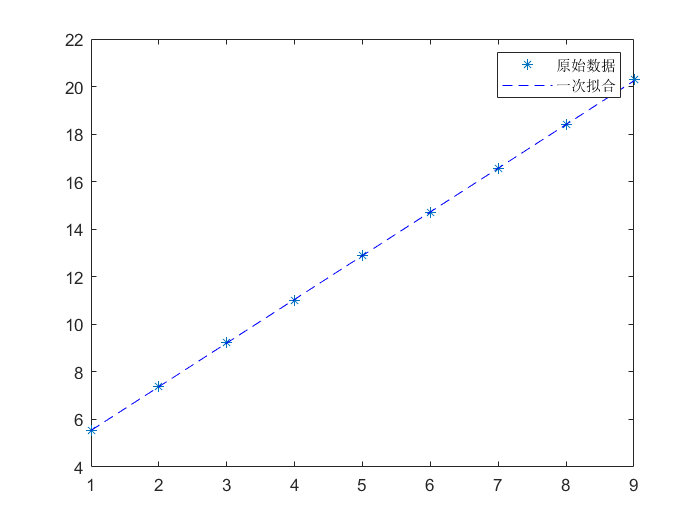
\includegraphics[width=3.5in]{water.png}
		\end{figure}
		
		经过matlab的计算得出斜率为1.8380,即取$\Delta x$=1.838cm.已知光的波长为$\lambda_l$=633nm,则$\lambda=\dfrac{\lambda_l}{\sin\theta}$,而$\tan\theta=\dfrac{\Delta x}{L}$,最后算出$v\approx 1500m/s$.

\subsection*{【误差分析】}
	\subsubsection*{1.极值法测量空气中声速}
	利用隔五项逐差法处理表一中的数据得到下表:
	\begin{table}[htbp]
	\centering
	\begin{tabular}{|c|c|c|c|c|c|}
	\hline
	\textbf{}&\textbf{1}&\textbf{2}&\textbf{3}&\textbf{4}&\textbf{5} \\
	\hline
	$\Delta x_i(mm)$ & 22.885 & 22.402 & 22.215 & 22.316 & 21.861 \\
	\hline
	$\Delta x_i^{\prime}(mm)$ & 21.861 & 22.026 & 21.879 & 22.018 & 22.919 \\
	\hline
	\end{tabular}
	\end{table}
	\par
	现将$\Delta x_i$和$\Delta x_i^{\prime}$统一为$\Delta$,则$\bar{\Delta}=(22.885+22.402+22.215+22.316+21.861+21.861+22.026+21.879+22.018+22.919)\div 10=22.2382(mm)$,而$\sigma_{\bar\Delta}=\sqrt{\dfrac{\sum_{i=1}^{10}(\Delta_i-\bar\Delta)^2}{10\times 9}}\approx 0.126(mm)$.\par
	若考虑仪器允差$e=0.004mm$,$\Delta$的总不确定度为
	\begin{equation*}
	\sigma_{\Delta}=\sqrt{\sigma_{\bar\Delta}^2+\frac{e^2}{3}}=\sqrt{(0.126)^2+\frac{(0.004)^2}{3}}=0.126(mm)
	\end{equation*}
	则有
	\begin{equation*}
	\Delta=\bar\Delta\pm \sigma_{\Delta}=(22.238\pm 0.126)mm
	\end{equation*}
	又由于$\lambda=\frac{2}{5}\Delta$,则$\sigma_{\lambda}=\frac{2}{5}\sigma_{\Delta}=0.4\times 0.126=0.0504(mm)=0.05(mm)$,则$\lambda=(8.90\pm0.05)mm$.最后测出声速为
	\begin{equation*}
	v=f_o\times\lambda=(348\pm2)m/s
	\end{equation*}
	
	\subsubsection*{2.相位法测量空气中声速}
	利用最小二乘法来分别处理两组数据,对第一组数据进行处理,得出斜率为$k_1=8.8494$,图像如下:
	\begin{figure}[htbp]
		\centering
		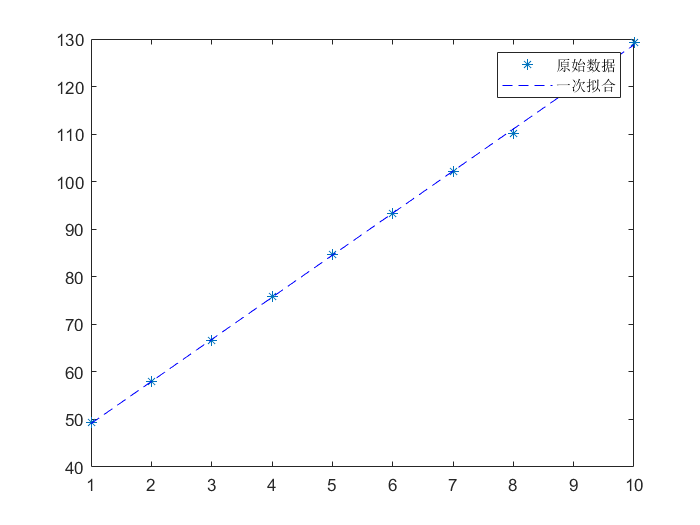
\includegraphics[width=3.5in]{xiang1.png}
		\end{figure}

	再处理第二组数据,得出斜率为$k_2=-8.8288$,图像如下:
	\begin{figure}[htbp]
		\centering
		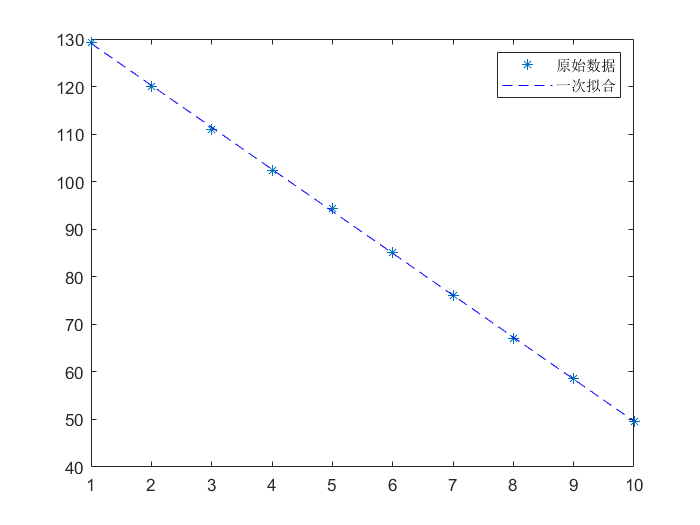
\includegraphics[width=3.5in]{xiang2.png}
		\end{figure}
		\par
	对于$y=kx+b$来说,$\sigma_k=\dfrac{\sigma_y}{\sqrt{\sum_{i=1}^{10}(i-5.5)^2}}$,且$\sigma_y=\dfrac{e}{\sqrt{3}}$,则有:
	\begin{gather*}
	\sigma_{k_1}=\dfrac{\frac{e}{\sqrt{3}}}{\sqrt{\sum_{i=1}^{10}(i-5.5)^2}}=0.0003(mm) \\
	\sigma_{k_2}=\dfrac{\frac{e}{\sqrt{3}}}{\sqrt{\sum_{i=1}^{10}(i-5.5)^2}}=0.0003(mm) \\
	k_1=(8.8494\pm0.0003)mm \\
	k_2=(-8.8288\pm0.0003)mm
	\end{gather*}
	又由于斜率的绝对值即为$\lambda$,则
	\begin{gather*}
	v_1=(346.20\pm0.01)m/s \\
	v_2=(345.39\pm0.01)m/s
	\end{gather*}
	
	\subsubsection*{3.气体参量法测空气中声速}
	由前可知,$v=331.45 \sqrt{(1+\dfrac{\theta}{273.15})(1+\dfrac{0.3192p_{s}H}{p})}$,根据方和根合成公式
	\begin{equation*}
	\sigma_v=\sqrt{[(\frac{\partial v}{\partial \theta}\sigma_{\theta})^2+(\frac{\partial v}{\partial H} \sigma_{H})^2+(\frac{\partial v}{\partial p} \sigma_{p})^2]}
	\end{equation*}
	\par
	又有如下关系:
	\begin{gather*}
	\sigma_{\theta}=\frac{1}{\sqrt{3}} \\
	\sigma_H =\frac{0.01}{\sqrt{3}} \\
	\sigma_p=\frac{0.05}{\sqrt{3}}
	\end{gather*}
	\\
	得出$\sigma_v=0.35(m/s)\approx 0.4(m/s)$,则$v=(347.3\pm0.4)m/s$.
	
	\subsubsection*{4.总结}
	\begin{enumerate}[(1)]
	\item 对于逐差法的不确定度分析来说,是一个求平均数和标准差的一个过程;而对于最小二乘法的不确定度分析来说,是一个不用求平均值标准差的过程,因为其$\sigma$的值是由仪器允差计算而来.则对于数据量过大的数据分析来说,利用最小二乘法的不确定度分析无疑是比较好的,因为不用去计算平均值的标准差,但是论精准度,那么一步一步地求取平均值和其标准差是较好的办法.
	\item 对于极值法和相位法测量的数据来说,与真实值的差别还是有一点,不确定度的有效数字皆为1,但是所处的数字位不一样,真实值的不确定度处于十分位,而极值法的处于个位,相位法的处于百分位.究其原因,可能是测量中具有随机误差,由于示波器显示在振幅处比较密集,在转动轮盘、读取数据时会有一定的随机误差;也有可能是在计算不确定的过程中出现的问题,在相位法中只进行了仪器允差的计算,而仪器允差毕竟属于系统误差,而在极值法中却考虑了系统误差和随机误差的双重影响.
	\end{enumerate}
	\subsection*{【思考题】}
	\begin{enumerate}[(1)]
	\item 能用人耳可听到的声音作为发射波吗?\par
	答:不能.在实验中有亲身经历,在调节信号发生器的频率时,在低频段,会有尖锐的蜂鸣声,但是CH-2所代表的曲线(即输出曲线)并没有明显波动,等到高频部分,人耳听不到的时候,CH-2代表的曲线才有了正弦波的样子.究其原因,是当频率在人耳范围内时,能量不足以使示波器显示出正常波形.
	\item 如何手动调整示波器方便极值和图像读取?\par
	答:可以将示波器的显示波形切换到持续模式,这样在调节$l$时,示波器上显示的波形会留有痕迹,根据这些痕迹可以大致判断出极值点在哪里,再根据$V_{pp}$值的大小,精准判断出极值点的所在位置.
	\item 如何估算和测量回程差的大小?\par
	答:在量程范围内测量,并画出上行和下行曲线,则回程差是两曲线的最大差值.
	\item 驻波和行波两个原理为什么可以共用?\par
	答:因为驻波是两列行波叠加而成.
	\item 极值出现的位置和相位法中的相位差有什么关系?实际测量中是否符合预期?\par
	答:相邻两个极值出现的位置之差是相位差的一半.在实际测量中也是这样的.
	\item 极值法中多极值出现的原因是什么?\par
	答:因为测量的是刚性平面处的声压强度,在移动$l$时,刚性平面处的声压会周期性变化,但是由于距离在改变,能量在中间部分的空气中会耗散掉一部分,则在两个不同的位置处,极值也是不一样的,根据表一也能看出来多极值的情况.
	\end{enumerate}
	
	
\end{document}
	
	
	
	
	
	
	 
	
	
	
	
	
	
	
	
	
	
	
	
	
	